%%%%%%%%%%%%%%%%%%%%%%%%%%%%%%%%%%%%%%%%%%%%%%%%%%%%%%%%%%%%%%%%%%%%
% bare_jrnl.tex
% V1.4b
% 2015/08/26
% by Michael Shell
% see http://www.michaelshell.org/
% for current contact information.                                                                 
%%%%%%%%%%%%%%%%%%%%%%%%%%%%%%%%%%%%%%%%%%%%%%%%%%%%%%%%%%%%%%%%%%%%

%% This is a skeleton file demonstrating the use of IEEEtran.cls
%% (requires IEEEtran.cls version 1.8b or later) with an IEEE
%% journal paper.
%%
%% Support sites:
%% http://www.michaelshell.org/tex/ieeetran/
%% http://www.ctan.org/pkg/ieeetran
%% and
%% http://www.ieee.org/


\documentclass[journal]{IEEEtran}
%
\usepackage{instructivo}  % Commands for multiple choice
\graphicspath{{./}{./fig/}}

\usepackage[natbib=true,style=trad-unsrt,backend=biber]{biblatex}

\addbibresource{literatura.bib}
\usepackage{circuitikz}
\usepackage{float}

% correct bad hyphenation here
\hyphenation{op-tical net-works semi-conduc-tor}


\begin{document}
%
% paper title
% Titles are generally capitalized except for words such as a, an, and, as,
% at, but, by, for, in, nor, of, on, or, the, to and up, which are usually
% not capitalized unless they are the first or last word of the title.
% Linebreaks \\ can be used within to get better formatting as desired.
% Do not put math or special symbols in the title.
\title{Experimento 02: Aplicaciones del Diodo}


\author{Juan~P.~Elizondo~Espinoza,~\IEEEmembership{Estudiante,~TEC}
        y~Matías~A.~Camacho~Abarca,~\IEEEmembership{Estudiante,~TEC.}
}


% The paper headers
\markboth{TEC.~EL-3215 Laboratorio de Electrónica Analógica, IS~2025}%
{EL3215 Laboratorio de Electrónica Analógica}


% make the title area
\maketitle


\begin{abstract}
El resumen no debe de exceder de 150 palabras y debe establecer lo que fue hecho, como fue hecho, los resultados principales y su significado. No cite referencias en el resumen. No coloque ecuaciones, símbolos especiales o palabras claves.
\end{abstract}

% Se sugiere no más de cuatro palabras o frases cortas en orden alfabético, separadas por comas, que representen su reporte
\begin{IEEEkeywords}
Diodo, tensión, corriente, junta, ruptura.
\end{IEEEkeywords}


%%%%%%%%%%%%%%%%%%%%%%%%%%%%%%%%%%%%%%%%%%%%%%%%%%%%%%%%%%%%%%%%%%%%%%%%%%%%%%%%%%%%%%%%%%%%%%
%%%%%%%%%%%%%%%%%%%%%%%%%%%%%%%%%%%%%%%%%%%%%%%%%%%%%%%%%%%%%%%%%%%%%%%%%%%%%%%%%%%%%%%%%%%%%%
\section{Introducción}

\IEEEPARstart{E}{n} esta sección se describe una introducción que le permita al lector identificar aspectos importantes para la comprensión de la lectura del documento, una visión relacionada al experimento y a los conocimientos científicos estudiados.


%%%%%%%%%%%%%%%%%%%%%%%%%%%%%%%%%%%%%%%%%%%%%%%%%%%%%%%%%%%%%%%%%%%%%%%%%%%%%%%%%%%%%%%%%%%%%%
%%%%%%%%%%%%%%%%%%%%%%%%%%%%%%%%%%%%%%%%%%%%%%%%%%%%%%%%%%%%%%%%%%%%%%%%%%%%%%%%%%%%%%%%%%%%%%
\section{Circuitos recortadores con Diodos}
El texto va aquí. La ecuación de la ley de Ohm es $V=I\cdot R$.


\subsection{Circuitos de Medición}

El circuito de la Fig. \ref{fig:recortador_sinDiodo} se utiliza para ver el comportamiento de la señal de salida (modificada por medio de un divisor de tensión), respecto a la señal de entrada Vs.

\begin{figure}[H]
        \centering
        \begin{circuitikz}
                % Fuente de señal CA
                \draw (0,0) to [sV, l=$Vs$] (0,2.5);
                \draw (0,2.5) to [short] (2.5,2.5);

                % Resistencia en paralelo a la fuente
                \draw (2.5,2.5) to [R, l=$R_1$] (2.5,0);

                % Resistencias en serie
                \draw (2.5,2.5) to [R, l^=$R_2$] (5,2.5);
                \draw (5,2.5) to [R, l=$R_L$] (5,0);

                \draw (5,0) to [short] (0,0);
        \end{circuitikz}
        \caption{Circuito recortador sin Diodo}
        \label{fig:recortador_sinDiodo}
\end{figure}

Luego, se modifica el circuito anterior al agregarle un diodo, de manera que ahora es un circuito recortador que utiliza un elemento activo. Según se muestra en la Fig. \ref{fig:recortador_conDiodo}.

\begin{figure}[H]
        \centering
        \begin{circuitikz}
                % Fuente de señal CA
                \draw (0,0) to [sV, l=$Vs$] (0,2.5);
                \draw (0,2.5) to [short] (2,2.5);

                % Resistencia
                \draw (2,2.5) to [R, l=$R_1$] (2,0);
                \draw (2,2.5) to [R, l^=$R_2$] (4.5,2.5);
                \draw (4.5,2.5) to [short] (6.5,2.5);
                \draw (6.5,2.5) to [R, l=$R_L$] (6.5,0);
                \draw (6.5,0) to [short] (0,0);


                % Diodo IN914
                \draw (4.5,2.5) to [D, l=$D_1$, fill=black] (4.5,0);

        \end{circuitikz}
        \caption{Circuito recortador con Diodo}
        \label{fig:recortador_conDiodo}
\end{figure}

Como tercera modificación, se le agrega una fuente en CD en serie con el diodo al circuito según la Fig. \ref{fig:recortador_conAjuste}, que agrega un ajuste a la tensión vista por la carga. 

\begin{figure}[H]
        \centering
        \begin{circuitikz}
                % Fuente de señal CA
                \draw (0,0) to [sV, l=$Vs$] (0,2.5);
                \draw (0,2.5) to [short] (2,2.5);

                % Resistencia
                \draw (2,2.5) to [R, l=$R_1$] (2,0);
                \draw (2,2.5) to [R, l^=$R_2$] (4.5,2.5);
                \draw (4.5,2.5) to [short] (6.5,2.5);
                \draw (6.5,2.5) to [R, l=$R_L$] (6.5,0);
                \draw (6.5,0) to [short] (0,0);


                % Diodo IN914
                \draw (4.5,2.5) to [D, l=$D_1$, fill=black] (4.5,1.25);

                % Fuente de CD
                \draw (4.5,1.25) to [battery, l=$V_{CD}$] (4.5,0);
                

        \end{circuitikz}
        \caption{Circuito recortador con Diodo con ajuste}
        \label{fig:recortador_conAjuste}
\end{figure}

\subsection{Simulaciones}
Acá se muestran y describen los resultados teóricos esperados por medio de simulaciones, para este caso corresponden a gráficas de señales en su mayoría. 


\subsection{Resultados Experimentales}

La gráfica de la Fig. \ref{fig:plot3} muestra una mala relación de tamaño para este formato de artículo, sin embargo, la que se muestra en la Fig. \ref{fig:plot4} se observan mejor los detalles de nombres de ejes y mayor resolución.

\begin{figure}[!ht]
\centering
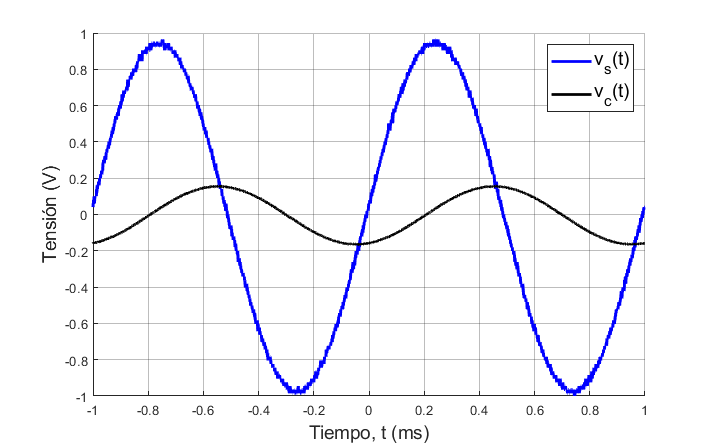
\includegraphics[width=3.7in]{plot4}
\caption{Tensión de entrada $v_s(t)$ y salida $v_c(t)$ de un filtro RC (versión 1)}
\label{fig:plot3}
\end{figure}

\begin{figure}[!ht] 
\centering
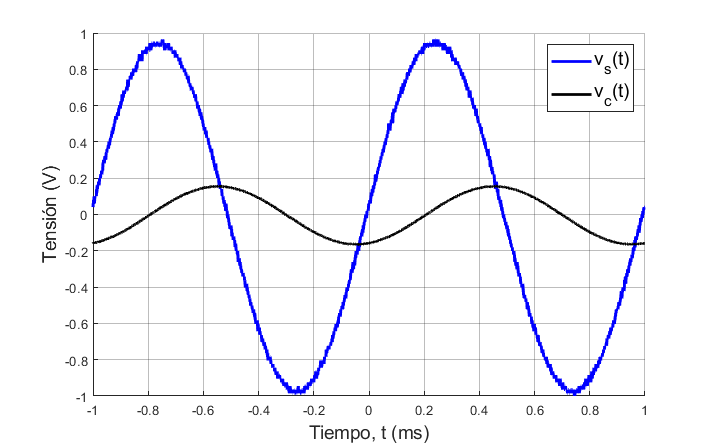
\includegraphics[width=3.7in]{plot4}
\caption{Tensión de entrada $v_s(t)$ y salida $v_c(t)$ de un filtro RC (versión 2)}
\label{fig:plot4}
\end{figure}

En la Tabla \ref{tabla1} se muestran los valores de resistencias utilizadas para realizar las mediciones del circuito de la Fig. \ref{fig:poldiodo}.

\begin{table}[!ht]
        \centering
        \caption{Valores de resistencia utilizados}
        \begin{tabular}{|>{\centering\arraybackslash}m{2cm}|>{\centering\arraybackslash}m{2cm}|>{\centering\arraybackslash}m{2cm}|}
             \hline
             Componente & Valor requerido & Valor medidido \\ 
             \hline
             $R_1$ & $330\,\Omega$& \\ 
             \hline
             $R_2$ & $1\,M\Omega$ & \\
             \hline
            \end{tabular}
    	\label{tabla1}   
	\end{table}


\vspace{5mm}

\subsection{Análisis de Resultados}
En el texto del documento usualmente se anotan citas bibliográficas, en donde la forma de hacerlo es la siguiente:


La tensión de ruptura del diodo se puede aproximar en $0.7\,$V \cite{Malik1996,Boylestad,Horowitz1989,Gray1995}. Por otro lado, la tensión de ruptura se puede considerar de $-40\,$V \cite{Floyd2008,Behzad2013,Schilling1994}. Un diodo puede considerarse como una junta de dos materiales, uno con un dopado de portadores mayoritarios mayor al otro material de la junta \cite{Pierret1994}.\\


La ecuación que describe la ley de Ohm es:
\begin{equation}
	V=I\cdot R
\end{equation}

%%%%%%%%%%%%%%%%%%%%%%%%%%%%%%%%%%%%%%%%%%%%%%%%%%%%%%%%%%%%%%%%%%%%%%%%%%%%%%%%%%%%
%%%%%%%%%%%%%%%%%%%%%%%%%%%%%%%%%%%%%%%%%%%%%%%%%%%%%%%%%%%%%%%%%%%%%%%%%%%%%%%%%%%%
\section{Graficando la Curva Característica del Diodo con el Osciloscopio}
El texto va aquí.

\subsection{Circuitos de Medición}
El circuito de la Fig. \ref{fig_cir2} se utiliza para o.

\begin{figure}[!ht]
\centering
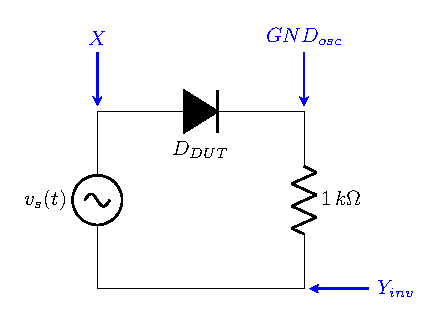
\includegraphics[width=3in]{circuito_3}
\caption{Circuito de polarización inversa}
\label{fig_cir2}
\end{figure}

\subsection{Simulaciones}
\subsection{Resultados Experimentales}


%%%%%%%%%%%%%%%%%%%%%%%%%%%%%%%%%%%%%%%%%%%%%%%%%%%%%%%%%%%%%%%%%%%%%%%%%%%%%%%%%%%%
%%%%%%%%%%%%%%%%%%%%%%%%%%%%%%%%%%%%%%%%%%%%%%%%%%%%%%%%%%%%%%%%%%%%%%%%%%%%%%%%%%%%
\section{Conclusiones}
Las conclusiones van aquí.

%%%%%%%%%%%%%%%%%%%%%%%%%%%%%%%%%%%%%%%%%%%%%%%%%%%%%%%%%%%%%%%%%%%%%%%%%%%%%%%%%%%%
%%%%%%%%%%%%%%%%%%%%%%%%%%%%%%%%%%%%%%%%%%%%%%%%%%%%%%%%%%%%%%%%%%%%%%%%%%%%%%%%%%%%
\appendices
\section{Demostración de la Ley de Ohm}
El texto relacionado al apéndice va aquí.

\section{Cálculos de polarización CD}
El texto relacionado al apéndice va aquí.



%%%%%%%%%%%%%%%%%%%%%%%%%%%%%%%%%%%%%%%%%%%%%%%%%%%%%%%%%%%%%%%%%%%%%%%%%%%%%%%%%%%%
%%%%%%%%%%%%%%%%%%%%%%%%%%%%%%%%%%%%%%%%%%%%%%%%%%%%%%%%%%%%%%%%%%%%%%%%%%%%%%%%%%%%
\section{}
\printbibliography


%%%%%%%%%%%%%%%%%%%%%%%%%%%%%%%%%%%%%%%%%%%%%%%%%%%%%%%%%%%%%%%%%%%%%%%%%%%%%%%%%%%%
%%%%%%%%%%%%%%%%%%%%%%%%%%%%%%%%%%%%%%%%%%%%%%%%%%%%%%%%%%%%%%%%%%%%%%%%%%%%%%%%%%%%
\begin{IEEEbiography}[{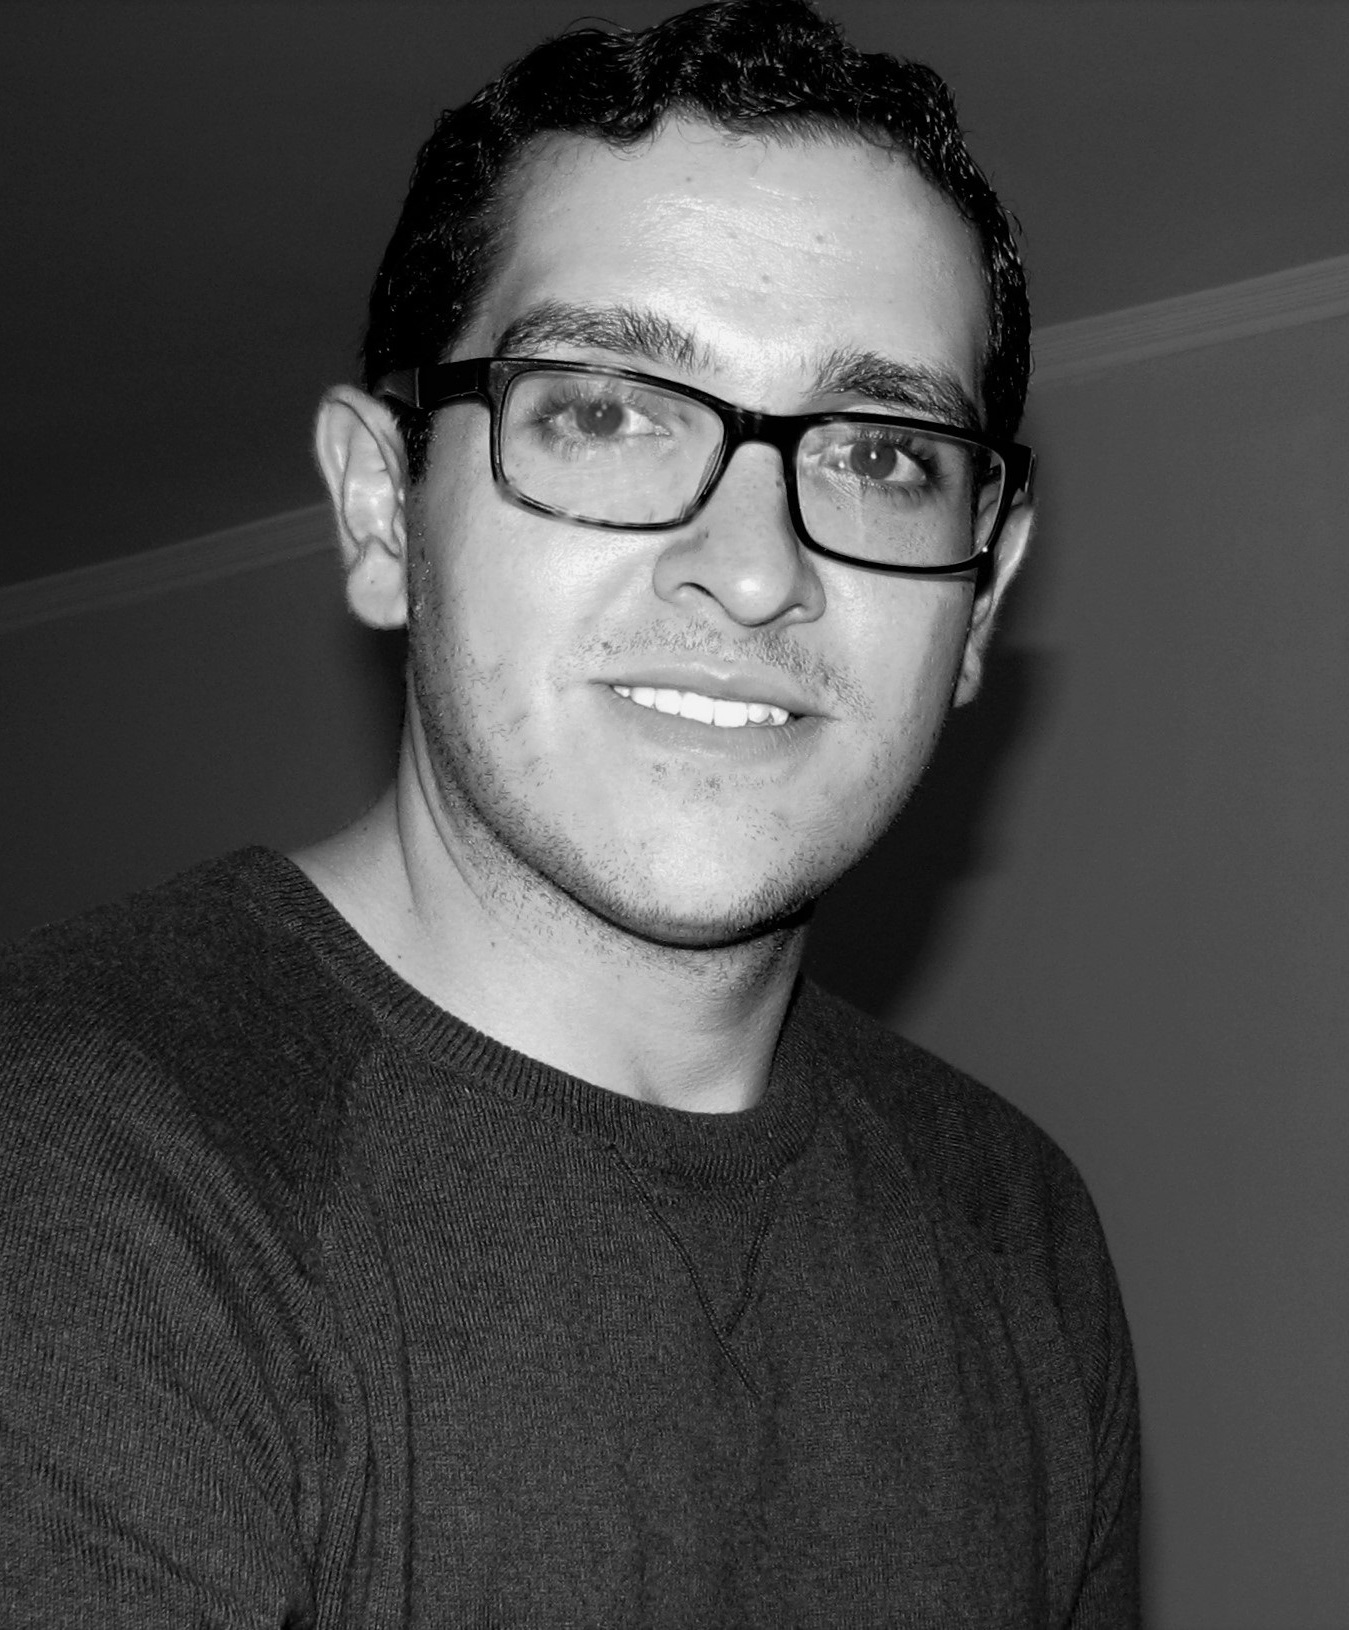
\includegraphics[width=1.05in,height=1.6in,clip,keepaspectratio]{cvjmv2}}]{José Miguel Barboza-Retana}

Ingeniero en electrónica con maestría científica en Sistemas Microelectromecánicos (MEMS). Profesor e investigador universitario de la Escuela de Ingeniería Electrónica con experiencia en los cursos de: Circuitos Eléctricos en CA, Laboratorio de Electrónica Analógica, Circuitos Integrados Analógicos, Señales y Sistemas y Procesamiento Digital de Señales. Además, cuenta con experiencia en proyectos de investigación relacionados en áreas biomédicas con conocimiento de simulación multifísica, sistemas microfluídicos y espectroscopía por impedancia eléctrica.
Correo: jmbarboza@itcr.ac.cr

\end{IEEEbiography}
 
% if you will not have a photo at all:
\begin{IEEEbiographynophoto}{Ronald Barboza-Retana}
Ingeniero en electrónica con maestría científica en Sistemas Microelectromecánicos (MEMS). Profesor e investigador universitario de la Escuela de Ingeniería Electrónica con experiencia en los cursos de:

\begin{itemize}
\item Circuitos Eléctricos en CA
\item Laboratorio de Electrónica Analógica
\item Circuitos Integrados Analógicos
\item Señales y Sistemas
\item Procesamiento Digital de Señales
\end{itemize} 

Correo: jmbarboza@itcr.ac.cr
\end{IEEEbiographynophoto}

\vfill

\end{document}